\chapter{What is a Proof?}
\begin{pr}\leavevmode
    \begin{enumerate}[label=\textbf{(\alph*)}]
        \item Colors of the triangles are arbitrary since I
        do not remember the exact ones in the text.
        \vspace{1cm}

        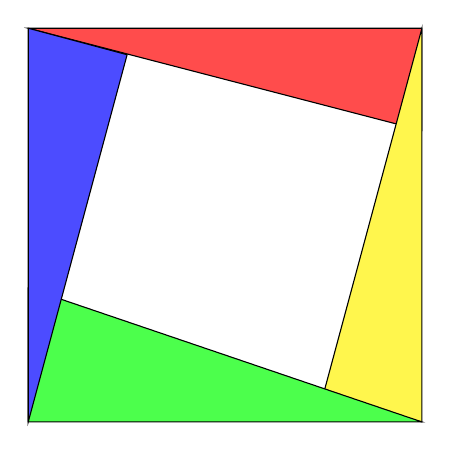
\begin{tikzpicture}
            \draw[fill=red!70] (0,0) -- (5,0) -- ++(-90:1.3) -- cycle;
            \draw[fill=yellow!70] (5,0) -- (5,-5) -- ++(165: 1.3) -- cycle;
            \draw[fill=green!70] (5,-5) -- (0,-5) -- ++(90:1.7) -- cycle;
            \draw[fill=blue!70] (0,-5) -- (0,0) -- ++(-15:1.3) -- cycle;
        \end{tikzpicture}

        \vspace{1cm}
        The middle square is a square of $(b-a) \times (b-a)$

        \item \note{Possible Errata:}
    \end{enumerate}
\end{pr}